\documentclass[a4paper]{letter}
\usepackage{wallpaper}
\usepackage{geometry}
\usepackage{xcolor}
\usepackage[T1]{fontenc}
\usepackage[scaled]{helvet}
\usepackage{fontawesome5}
\usepackage[hidelinks]{hyperref}
\usepackage[french]{babel}
\usepackage{graphicx}
\usepackage{tikz}
\usepackage{setspace}
\usepackage{comment}

\usetikzlibrary{calc}

\renewcommand{\familydefault}{\sfdefault}

\geometry{
  a4paper,
  left=20pt,
  right=20pt,
  top=0pt,
  bottom=0pt,
  nohead,
  nofoot,
  nomarginpar
}

\ThisCenterWallPaper{1.1}{cvbg.png}

% Custom command for dividers
\newcommand{\divider}{\rule{\linewidth}{0.9pt}}

% ============================================================
% ======================== Left Side =========================
% ============================================================


\begin{document}

%\small
\begin{minipage}[t]{0.40\textwidth}
\setstretch{1.2} 
\setlength{\baselineskip}{1\baselineskip}
\color{white}
\vspace{5mm}


% ========================== Photo ============================

\begin{tikzpicture}
    \clip (0,0) circle (2cm);
    \node[anchor=center] at (0,0) {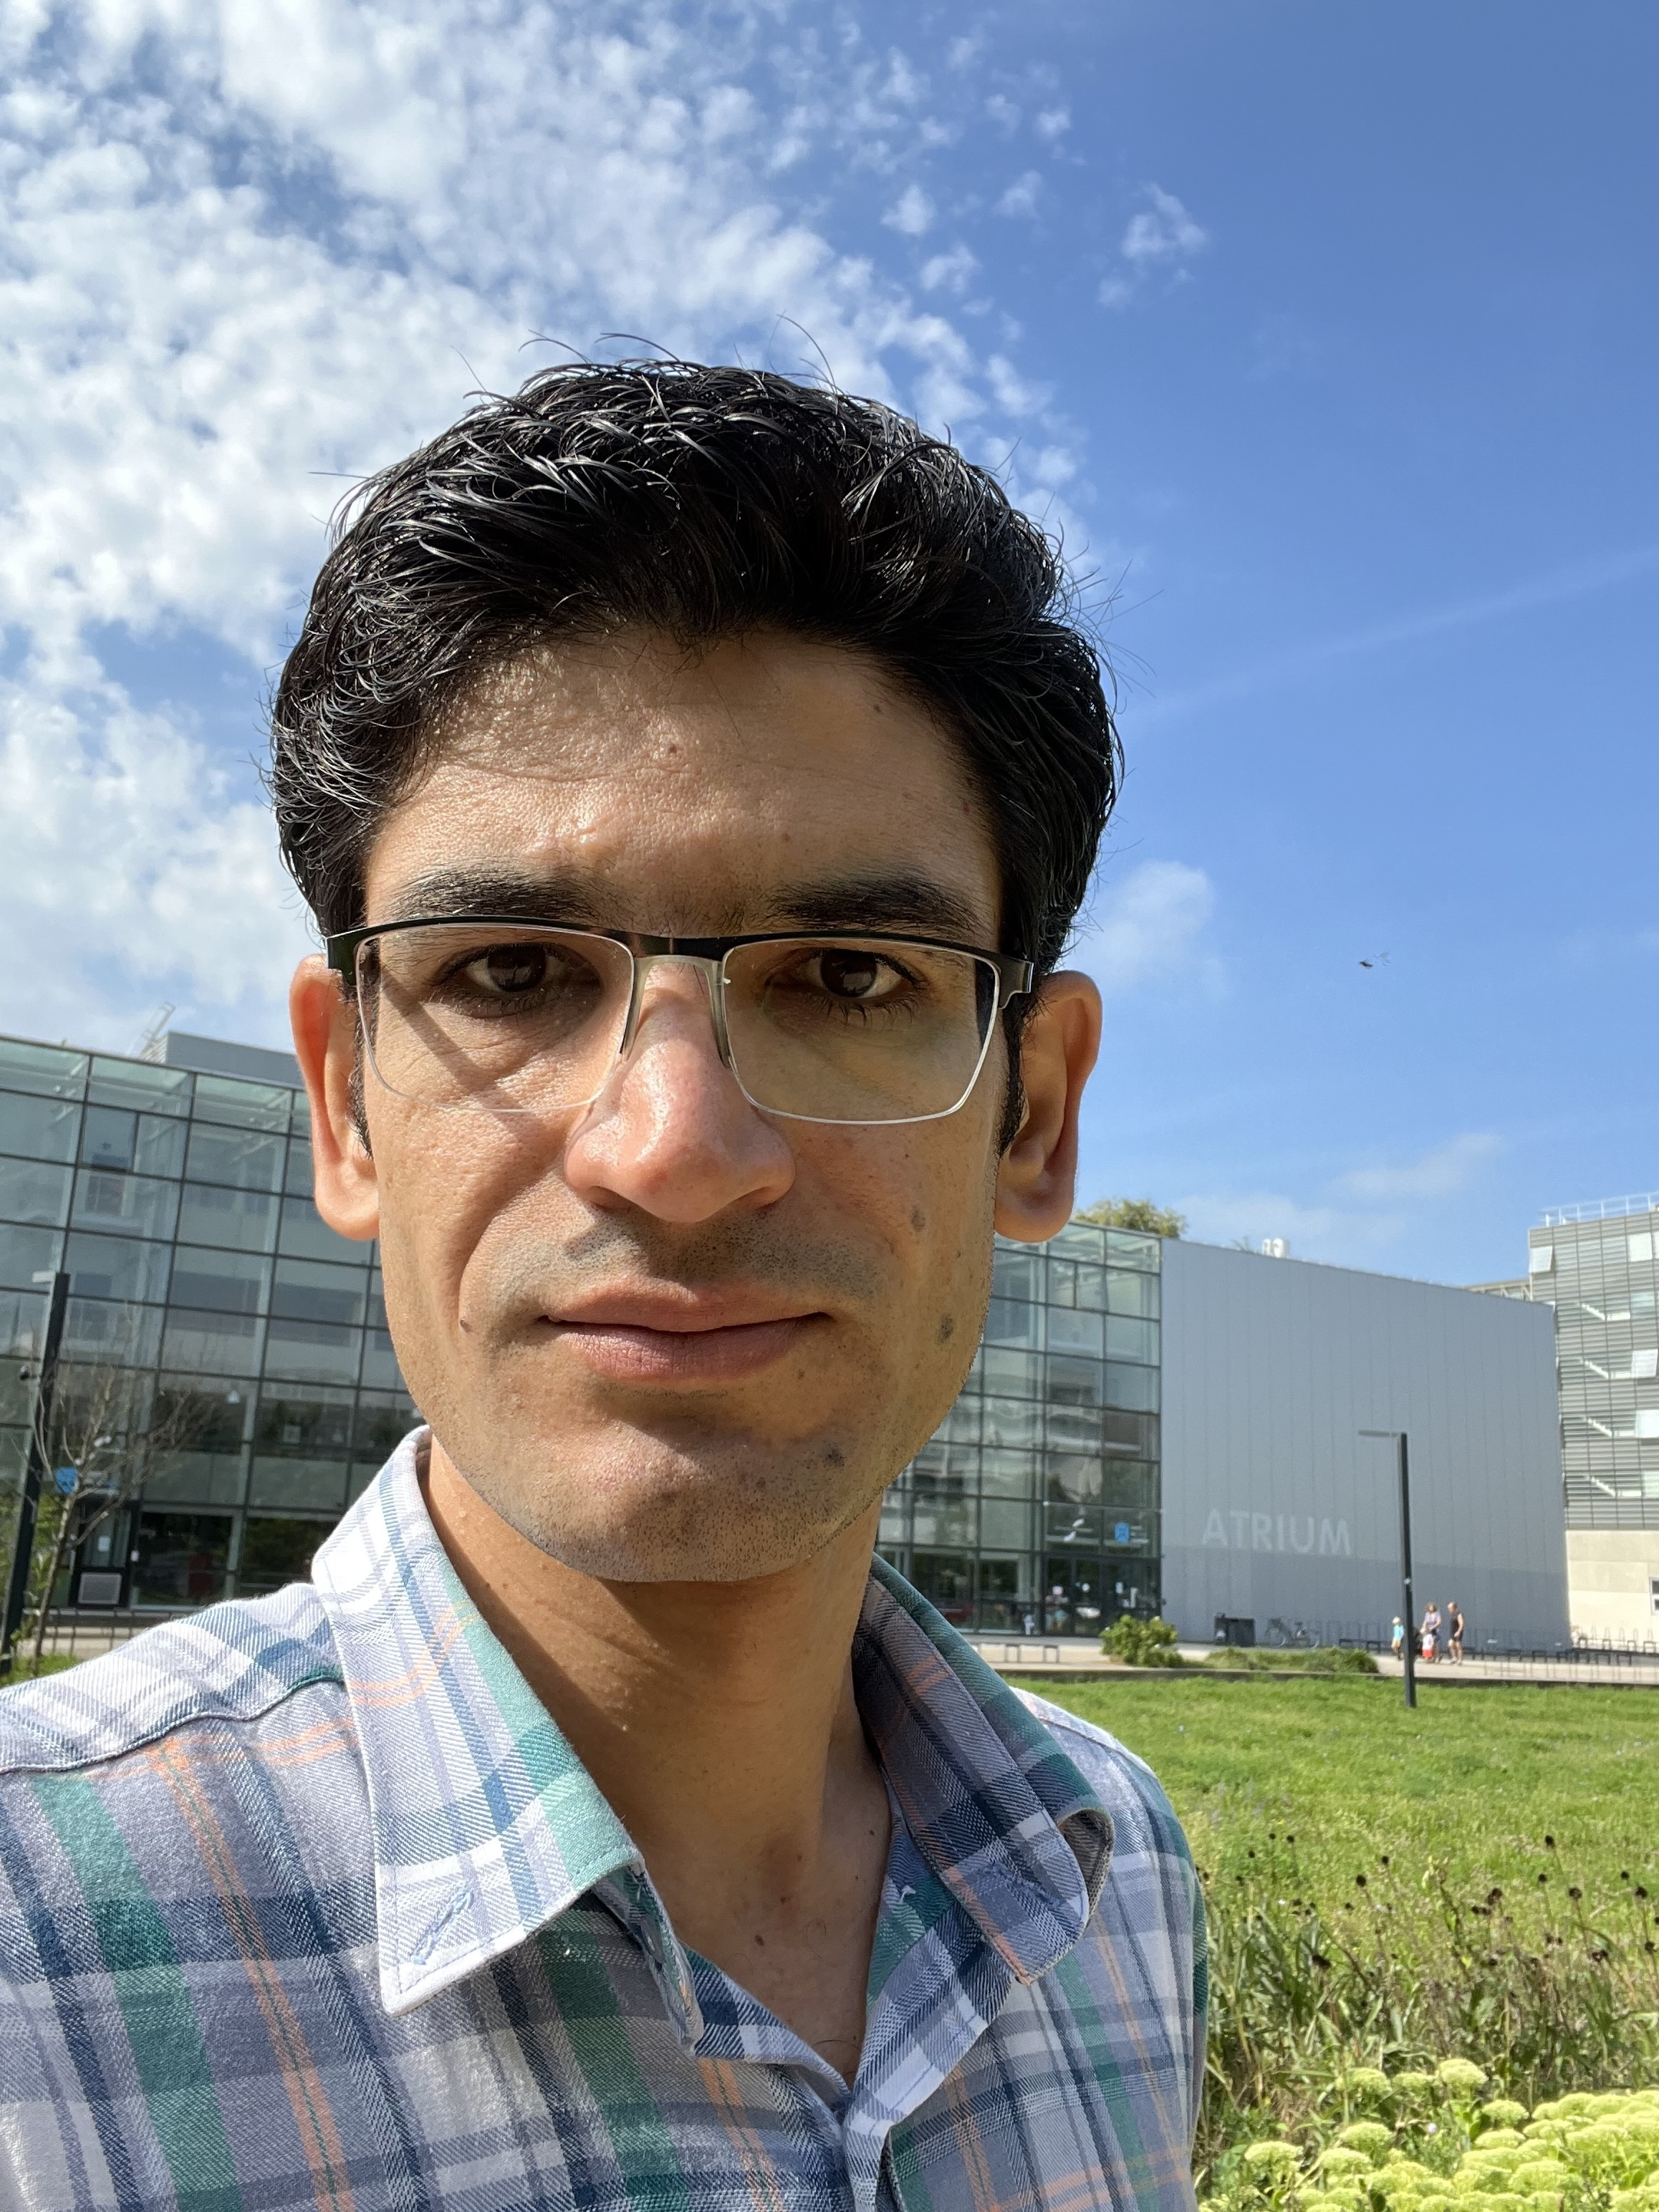
\includegraphics[width=4cm]{profile.jpg}};
\end{tikzpicture}

\vspace{5mm}

\divider

% ========================= Contact ===========================

\faPhone \quad 06 52 22 49 24

\faEnvelope \quad jafarizadeh89@gmail.com

\faGithub \quad \href{https://github.com/jafarizadeh}{jafarizadeh}

\faLinkedin \quad \href{https://www.linkedin.com/in/jafarizadeh/}{linkedin.com/in/jafarizadeh/}


\divider

% ================ Langues ================
{\large \textbf{Langues}}

\faCircleNotch \quad Persan (langue maternelle)

\faCircleNotch \quad Français (niveau avancé)

\faCircleNotch \quad Anglais (niveau intermédiaire)

\divider

% ================ Langage de Programmation ================

{\large \textbf{Langage de Programmation}}

\faCircleNotch \quad Python

\faCircleNotch \quad C

\faCircleNotch \quad Swift

\faCircleNotch \quad HTML / CSS

\faCircleNotch \quad JavaScript

\faCircleNotch \quad SQL

\divider

% ===================== Logiciel de CAO ======================

{\large \textbf{Logiciel de CAO}}

\faCircleNotch \quad AutoCAD

\faCircleNotch \quad CATIA

\divider

% ========================== Réseau ==========================


{\large \textbf{Réseau}}

\faNetworkWired \quad CCNP-ENCOR (en cours)

\faNetworkWired \quad CCNP-ENARSI

\faNetworkWired \quad CCNA


\divider
% ===================== Permis de Conduire ======================

{\large \textbf{Permis de Conduire}}

\faCar \quad Permis B2

\divider
% ===================== Centres d'intérêt ======================

{\large \textbf{Centres d'intérêt}}

\faBicycle \quad vélo

\faGamepad \quad jeux vidéo (Minecraft)


\end{minipage}
\hfill
\begin{minipage}[t]{0.60\textwidth}




% ============================================================
% ======================= Right  Side ========================
% ============================================================

\setlength{\baselineskip}{1.5\baselineskip}
\vspace{0.7cm}

{\huge Mehdi JAFARIZADEH}

\vspace{0.5cm}

% ========================= Éducation =========================

{\large \textbf{Éducation}}
\divider


{\textbf{Licence (3em année) en Informatique}}

{\footnotesize Septembre 2021 - Présent}

{\textit{Université de Strasbourg, Strasbourg}}

\vspace{1mm}

\begin{itemize}
    \footnotesize
    %\item Cours suivis et certifications :
        %\begin{itemize}
            
            %\item CCNA (Cisco Certified Network Associate) - udemy (128h)
            %\item ENARSI (Cisco Enterprise Advanced Routing and Services) - udemy (134h)
            %\item IT network cabling: The complete fiber optics course - udemy (19h)
            %\item Wireshark for Beginners: Capture et l'analyse de paquets réseau pour le diagnostic et le dépannage - coursera (2h)
        %\end{itemize}
    \item Compétences acquises : configuration et gestion de réseaux LAN/WAN, 
    gestion des processus, administration Linux, analyse de complexité, structures de données.
\end{itemize}

\vspace{3mm}


{\textbf{Bachelor en Génie des Énergies (équivalent Licence)}}

{\footnotesize Septembre 2014 - Décembre 2018}

{\textit{Université technologique de Quchan, Mashhad, Iran}}

\vspace{1mm}

\begin{itemize}
    \footnotesize
    \item Projet de fin d'études : Consommation énergétique des maisons intelligentes
    \item Compétences acquises : Modélisation énergétique, Optimisation de l'efficacité énergétique, Utilisation de logiciels spécialisés
\end{itemize}

\vspace{3mm}

{\textbf{Diplôme en Comptabilité (Bac+2)}}

{\footnotesize Septembre 2007 - Décembre 2010}

{\textit{Université Azad de Kerman, Kerman, Iran}}

\vspace{1mm}
\begin{itemize}


    \footnotesize
    \item Compétences acquises : Analyse financière, Conformité réglementaire
\end{itemize}
\vspace{3mm}
% ================ Formations Complémentaires ==================

{\large \textbf{Formations Complémentaires}}
\divider
\vspace{4mm}
\begin{itemize}
    \footnotesize \item {\textbf{CCNP ENCOR 350-401:} Architecture, sécurité, et automatisation d'infrastructure; (173 h)}
    \vspace{2mm}
    \footnotesize \item {\textbf{CCNP ENARSI 300-410:} Routage avancé EIGRP, OSPF, BGP et réseaux WAN; (134 h)}
    \vspace{2mm}
    \footnotesize \item {\textbf{CCNA 200-301:} Bases des réseaux, configuration et dépannage ; (128 h)}
\end{itemize}
\vspace{3mm}




% ================ Expérience Professionnelle =================


{\large \textbf{Expérience Professionnelle}}
\divider
    

\vspace{1mm}
{\textbf{Stage: Département informatique}}

{\footnotesize mai 2010 - Septembre 2010}
\begin{itemize}
    \footnotesize \item \textit{Cabinet de comptabilité Aria-Etemad}
   \newline
    Effectué des calculs de comptabilité client à l’aide de Microsoft Office, notamment Excel. Développé des compétences avancées en Microsoft 365 et en calculs comptables au cours de cette expérience.
\end{itemize}


\vspace{3mm}
{\textbf{Stage: Département recherche et développement}}

{\footnotesize Juin 2017 - Septembre 2017}
\begin{itemize}
    \footnotesize \item \textit{Industrie des câbles de Kerman et Kavian}
   \newline
    Mené des recherches sur l’analyse thermique et la conductivité électrique des fils de cuivre sous la supervision du Dr Abdollahi. Utilisé des outils tels qu’ANSYS et SolidWorks pour modéliser et analyser des données techniques. Effectué des études approfondies sur des articles scientifiques pour appuyer les travaux de recherche.
\end{itemize}


\vspace{3mm}
{\textbf{Directeur de l'association d'ingénierie énergétique}}

{\footnotesize Septembre 2015 - Décembre 2017}
\begin{itemize}
   \footnotesize \item \textit{Université technologique de Quchan, Mashhad}
   \newline
   Animé des cours pédagogiques et organisé des concours scientifiques au sein de l'Association d'ingénierie énergétique, pour promouvoir les énergies renouvelables et sensibiliser aux enjeux de l'efficacité énergétique.
\end{itemize}

\vspace{3mm}

{ \textbf{Assistant enseignant}}

{ \footnotesize Septembre 2014 - Décembre 2017}
\begin{itemize}
    \footnotesize \item \textit{Université technologique de Quchan, Mashhad}
    \newline
    Assistant enseignant en Mathématiques 1, Mathématiques 2 et Conversion énergétique : soutien aux étudiants, explication des concepts clés et aide à la préparation des travaux dirigés et des examens.
\end{itemize}


\vspace{3mm}


% ================ Projet ==================
\begin{comment}
{\large \textbf{Projets}}
\divider
\vspace{4mm}
\begin{itemize}
    \footnotesize \item {\textbf{Affichage et générateur de grille de mots croisés}, \textit{Développé une application Java pour générer, afficher et vérifier des grilles de mots croisés, en mettant en œuvre une architecture modulaire et des algorithmes de génération de grille et de vérification.}}
    \vspace{2mm}
    \footnotesize \item {\textbf{Graphe dual d’un maillage}, \textit{Développé en C un algorithme transformant un maillage en graphe dual et optimisé le tri des arêtes et la coloration avec Dijkstra.}}
    \vspace{2mm}
    \footnotesize \item {\textbf{web Programmation}, \textit{Conçu et développé un site portfolio en utilisant JavaScript et PHP, intégrant des fonctionnalités interactives et dynamiques.}}
    \vspace{2mm}
    \footnotesize \item {\textbf{EES}, \textit{Simulé et analysé une centrale électrique avec le logiciel EES, optimisant les performances énergétiques.}}


\end{itemize}

\vspace{3mm}
\end{comment}
% ================ Contributions Académiques ==================

{\large \textbf{Contributions Académiques}}
\divider
\vspace{3mm}
\begin{itemize}
    \footnotesize \item {\textbf{Co-auteur}, \textit{Guide d’audit énergétique pour les étudiants de l’Université de Quchan, avec Dr. Majid Mahdavian, Publié en 2019}}


\end{itemize}

% ================ Formations Complémentaires ==================

%{\large \textbf{Formations Complémentaires}}
%\divider
%\vspace{4mm}
%\begin{itemize}
    
    %\footnotesize \item {\textbf{CCNP ENARSI 300-410}, \textit{Formation CCNP ENARSI 300-410 : maîtrise avancée du routage et des services d'infrastructure réseau pour les environnements complexes.}}
    %\vspace{2mm}
    %\footnotesize \item {\textbf{CCNA 200-301}, \textit{Formation CCNA 200-301 : compétences fondamentales en réseaux, incluant la configuration, gestion et dépannage d'infrastructures réseaux.}}
    %\vspace{2mm}
    %\footnotesize \item {\textbf{Wireshark for Beginners: Capture Packets}, \textit{Formation Wireshark for Beginners : initiation à la capture et l'analyse de paquets réseau pour le diagnostic et le dépannage.}}
    %\vspace{2mm}
    %\footnotesize \item {\textbf{Initiation à Wireshark pour l’analyse de paquets sous linux}, \textit{Initiation à Wireshark : capture et analyse de paquets réseau sous Linux pour le diagnostic et la sécurité.}}
    %\vspace{2mm}
    %\footnotesize \item {\textbf{Configure VLANs on Cisco Switches}, \textit{Configuration de VLANs sur des commutateurs Cisco pour segmenter et sécuriser les réseaux.}}
    %\vspace{2mm}
    %\footnotesize \item {\textbf{Google Cloud Fundamentals: Core Infrastructure}, \textit{Formation Google Cloud Fundamentals : maîtrise des concepts clés de l'infrastructure cloud, y compris les services de calcul, de stockage et de gestion de réseau.}}
    

%\end{itemize}

%\vspace{3mm}


\end{minipage}

% ========================== Code QR ==========================

\begin{tikzpicture}[remember picture,overlay]
    \node[anchor=south east,inner sep=0pt] at ($(current page.south west)+(6.5cm,+2.5cm)$) {
        
\includegraphics[width=2cm]{Documentation_FR.png}
    };
    
    \node[anchor=south east,inner sep=0pt] at ($(current page.south west)+(4cm,+2.5cm)$) {
        \begin{minipage}[t]{3.05cm} 
            \color{white} \scriptsize \href{https://drive.google.com/file/d/1jKjZWYadaikaPetkEmjoupWWh_w1sMKA/view?usp=drive_link}{Veuillez cliquer ici ou scanner ce code QR pour accéder à un dossier détaillé de mes contributions académiques et professionnelles.}
        \end{minipage}
    };


    \node[anchor=south west,inner sep=0pt] at ($(current page.south west)+(0.8cm,1cm)$) {
        \begin{minipage}[t]{4cm}
            \tiny \textcolor{white}{Dernière mise à jour: \today}
        \end{minipage}
    };
\end{tikzpicture}

\end{document}
